\section{Introduction}

    Up until now, we have restricted the identification of excesses to within a 75~pc volume around the Sun. This is because stars within this volume have accurate parallaxes, and make excellent targets for further disk characterization through high-contrast imaging techniques. In addition, the stars have very little to no line-of-sight extinction from interstellar dust. These are stars within a structure known as the Local Bubble \citep{Lallement2003}. 
    
    However, the nearby solar neighborhood has been heavily scrutinized for debris disks by the last thirty years of disk detections, by missions from \iras, \spitzer, and now \WS. If one considers the census of debris disks within 120~pc, roughly 80\%  reside within a volume 75~pc, while only $\sim$20\% are within the volume between 75 and 120~pc. However, by looking at the distribution of \hip\ main-sequence stars within 120~pc, the ratio of stars between 0--75~pc and 75--120~pc is nearly 50/50. In addition, the density of stars increases at lower galactic lattitudes. However, only $\sim$8\% of known debris disks are within the galactic plane. Usually, the galactic plane is avoided because of the density of stars, which can cause source confusion and false detections. But if we are to believe the incidence rate of disks derived by the last thirty years of disk detections, there are a vast number of new debris disks that have yet to be identified, both beyond 75~pc, and within the galatic plane.
    
    %lit known 75: 606
    %lit 75-120: 161
    %lit total: 767
    %lit all : 1025
    %lit inside gal plane (5 deg): 77
    % percent disks within galactic plane: 
    
    
    
    Since we already have the necessary tools in place, and our parent sample of stars (see \S~2.2.1 in Chapter~\ref{chap:iddisks}) already extends out to 120~pc, it may seem like a relatively simple matter to merge the science and parent samples and identify excesses of the entire parent sample. Unfortunately, stars beyond 75~pc are more likely to be affected by line-of-sight extinction. The interstellar dust will decrease the intensity of shorter wavelength light from a star, thereby artificially boosting any measured mid-IR excess flux. Thus, an accurate assessment of an excess beyond 75~pc, for a large sample of stars, requires a priori knowledge of the extinction level for all our stars at the various \WS\ bands.
    
    To largely remove the effects of interstellar extinction, one can use the $W3$ and $W4$ bands to search for $W3-W4$ single color excesses. Interstellar extinction is greater at the $W1$ and $W2$ bands than at $W3$. In addition, the data show a relatively flat slope for the IR extinction curve between 10 and 20\micron\ \citep{Wang2014}. Thus, any extinction felt by $W3$ will be roughly of the same magnitude felt by $W4$, preserving the measured infrared excess flux. In this study, we investigate the presence of warm and faint excesses at $W4$ all the way out to 120~pc, by identifying significant $W3-W4$ color excesses. In addition, we include stars within the galactic plane by first removing stars contaminated from blended sources by using our astrometric offset analysis, which we introduced in \S~\ref{sec:auto_rejunwise}.
    

\section{Sample Selection}

    We used a subset of the sample of \hip\ stars used in \S~2 of Chapter~\ref{chap:iddisks}. To summarize, we selected main sequence \hip\ stars with well behaved \WS\ All-Sky photometry in the $W3$ and $W4$ bands. Our parent sample consists of stars within 120~pc with optical Tycho colors constrained to $-0.17~\rm{mag}< B_T-V_T< 1.4~\rm{mag}$ (late B to K spectral types). Since we are only interested in the $W3-W4$ colors for this study, saturation corrections to the $W1$ and $W2$ photometry were not necessary. Filters from \S~2.2.1 in Chapter~\ref{chap:iddisks}, that are relevant to the $W3$ and $W4$ bands, were placed on our parent sample of stars. 
    
    In contrast to the last two studies, here we include stars within the galactic plane. This adds an additional 766 \hip\ stars with well behaved $W3$ and $W4$ photometry to our parent sample, bringing the number of stars in our $W3-W4$ parent sample to 15199. We would also like to point out that in this study, we increase our science sample out to 120~pc. Therefore, our science and parent samples are equivalent.

   \subsection{Culling the Parent Sample via \textit{unWISE} Images}\label{sec:unwise_reject}
    
    The higher angular resolution \WS\ images from the \textit{unWISE} image service \citet{Lang2014} affords us the opportunity to identify sources that are potentially contaminated from blended point sources (e.g., active galactic nuclei, luminous infrared galaxies, other stars, etc.) or extended emission from interstellar IR nebulosity. Contaminated sources will manifest themselves as astrometric offsets, calculated from the centroid positions between the $W3$ and $W4$ images or by using different sized apertures in the $W4$ band to calculate the star's astrometric offset. In Chapter~\ref{chap:confirm}, our goal was to identify contaminants amongst the excesses we had already discovered. In contrast, here we aim to reject potentially contaminated stars \textit{prior} to excess identification.
    
    In short, we aimed to identify point source contamination by rejecting stars with significant $W3$ to $W4$ relative centroid offsets ($\Delta r_{W3,W4} = \left|\vec{r}_{_{W3}} - \vec{r}_{_{W4}}\right|$), as well as identify and reject stars contaminated from extend source emission from their $W4$ to wide-$W4$ centroid offsets ($\Delta r_{W4} = \left|\vec{r}_{_{W4}} - \vec{r}_{_{W4},_{wide}}\right|$). For this analysis, we extracted centroids for all the stars from their \textit{unWISE} $W3$ and $W4$ images. A detailed description of these procedures is discussed in \S~\ref{sec:unwise_rejectmethod}. 
    
    We looked for contaminated sources by identifying stars with statistically significant offsets. The density clouds in Figures~\ref{fig:unwise_w3w4} and \ref{fig:unwise_w4w4} show the distributions of 15304 stars from our $W3-W4$ parent sample, prior to applying the filters we placed in \S~2.2.1 of Chapter~\ref{chap:iddisks}. The plots show the distribution of our stars' $W4$ SNRs as a function of the $W3$ to $W4$ relative centroid offsets ($\Delta r_{W3,W4}$) as well as a function of the $W4$ to wide-$W4$ centroid offsets ($\Delta r_{W4}$). Low $W4$ SNR stars will be larely affected by small scale background variations, thus shifting the distribution at lower SNRs toward larger separations, while the opposite effect will occur for stars at higher SNRs. Thus, a natural upper envelope to the distribution arises, where stars above that envelope will be rejected. 
    
    %=============================================================
    % unWISE W3/W4
    %=============================================================
    \begin{figure}
    \centering
    \includegraphics[width=\textwidth]{Ch5/w3w4_snrvsep_galplane}
    \caption[Rejected \textit{unWISE} stars using $W3$ to $W4$ offsets]{Distribution of relative positional offsets of stellar centroids between $W3$ and $W4$ using images from the \textit{unWISE} image service, plotted with respect to the $W4$ SNR calculated from the \textit{unWISE} images. The black/gray density cloud represents the density of 15304 Hipparcos stars from the parent 120~pc sample. The black-dotted line represents our separation cut-off ($1/3$~pixels) below which stars are not rejected. Our rejection threshold (orange dotted line) was fit to $\{\Delta r_{j,max}\}$ (dark-blue diamonds), calculated as described in Section~ \ref{sec:unwise_rejectmethod}. Rejected stars to the right of the vertical dotted black line and above the orange dotted line (red squares) are deemed to be contaminated by an unrelated nearby point or extended source seen in projection.}
    \label{fig:unwise_w3w4}
    \end{figure}
    %=============================================================


    %=============================================================
    % unWISE W4/W4
    %=============================================================
    \begin{figure}
    \centering
    \includegraphics[width=\textwidth]{Ch5/w4w4_snrvsep_galplane}
    \caption[Rejected \textit{unWISE} stars using $W4$ to $W4$ offsets]{Distribution of relative positional offsets of stellar centroids between a narrow 2.5~pixel radius and wide 10~pixel radius apertures, as described in Section~\ref{sec:centroid_calc}. The plot elements are the same as those described in Figure~\ref{fig:unwise_w3w4}. Rejected parent sample stars are marked as red circle.}
    \label{fig:unwise_w4w4}
    \end{figure}
    %=============================================================
    
    The upper envelopes in both distributions were calculated by fitting an exponential curve to the $\Delta r_{j,max}$ points in log-log space, and using the same techniques outlined in \S~\ref{sec:unwise_rejectmethod} to calculate $\Delta r_{j,max}$. We also kept the same fixed 1/3~pixel lower limit for both analyses. In other words, stars are not rejected below this separation. The red points in Figures~\ref{fig:unwise_w3w4} and \ref{fig:unwise_w4w4} show stars from the parent sample that are likely contaminated by blended point sources or extended emission. Two hundred and twenty stars were rejected from the $\Delta r_{W3,W4}$ vs. $W4$ SNR analysis, and 738 stars were rejected from the $\Delta r_{W4}$ vs. $W4$ SNR analysis. The union of these two sets show that a total of 919 stars should be rejected, though only 897 stars from our filtered parent sample match the astrometric outliers. Out of the 897 rejected stars, 174 reside in the galactic plane, leaving 592 galactic plane stars in our parent sample. Our final $W3-W4$ parent sample is comprised of 14302 main-sequence \hip\ stars with well behaved $W3$ and $W4$ photometry.
    
    The 897 rejected stars account for 6.27\% of the original parent sample. Based on our assumptions, the photometry of all these stars must be contaminated by either extended emission or a blended point source. Though it is difficult to verify this claim, we show in the following section that the distribution of excess significances are much better behaved after removing these stars, implying to some extent that our analysis is doing a good job of cleaning the parent sample of stars.
    

\section{IR Excess Identification}

    Our excesses are selected using the same procedures described in \S~2.5 in Chapter~\ref{chap:iddisks} and the improved methods for identifying single-color excesses in \S~\ref{sec:improved_detection}. We use Equation~\ref{eq:old_sig}, to determine the significance of the color excess for each star. Since we only wish to identify excesses with $W3-W4$ colors only, the excess significance takes on the form of
    
    \begin{equation}\label{eq:excess_sig_w3-w4}
    \Sigma_{E[W3-W4]} = \frac{W3-W4-W_{34}(B_T-V_T)}{\sigma_{34}},
    \end{equation}

    \noindent where $W_{34}(B_T-V_T)$ is the empirically derived $W3-W4$ photospheric colors, and $\sigma_{34}$ is the total error term which includes the photometric and photospheric uncertainties. Both of these quantities are derived in \S~ in Chapter~\ref{chap:iddisks}. 
    
    Figure~\ref{fig:sige_w3-w4} shows the distribution of $\Sigma_{E[W3-W4]}$ for our parent sample of stars. We selected excesses such that their $\Sigma_{E[W3-W4]} \geq \Sigma_{E[W3-W4]_{99.5}}$. $\Sigma_{E[W3-W4]_{99.5}}$ is our 99.5\% confidence threshold, beyond which 0.5\% of stars are false-positive detections. In other words, our analysis is set to identify excesses up to a 99.5\% false-discovery rate (FDR). $\Sigma_{E[W3-W4]_{99.5}}$ was calculated using the same procedures that we describe in \S~\ref{sec:single_color_stuff}. For this analysis, we determined $\Sigma_{E[W3-W4]_{CL}}=2.894$, and is marked as the dotted black line n Figure~\ref{fig:sige_w3-w4}. 

    %=============================================================
    %  Color Distribution
    %=============================================================
    \begin{figure}
    \centering
    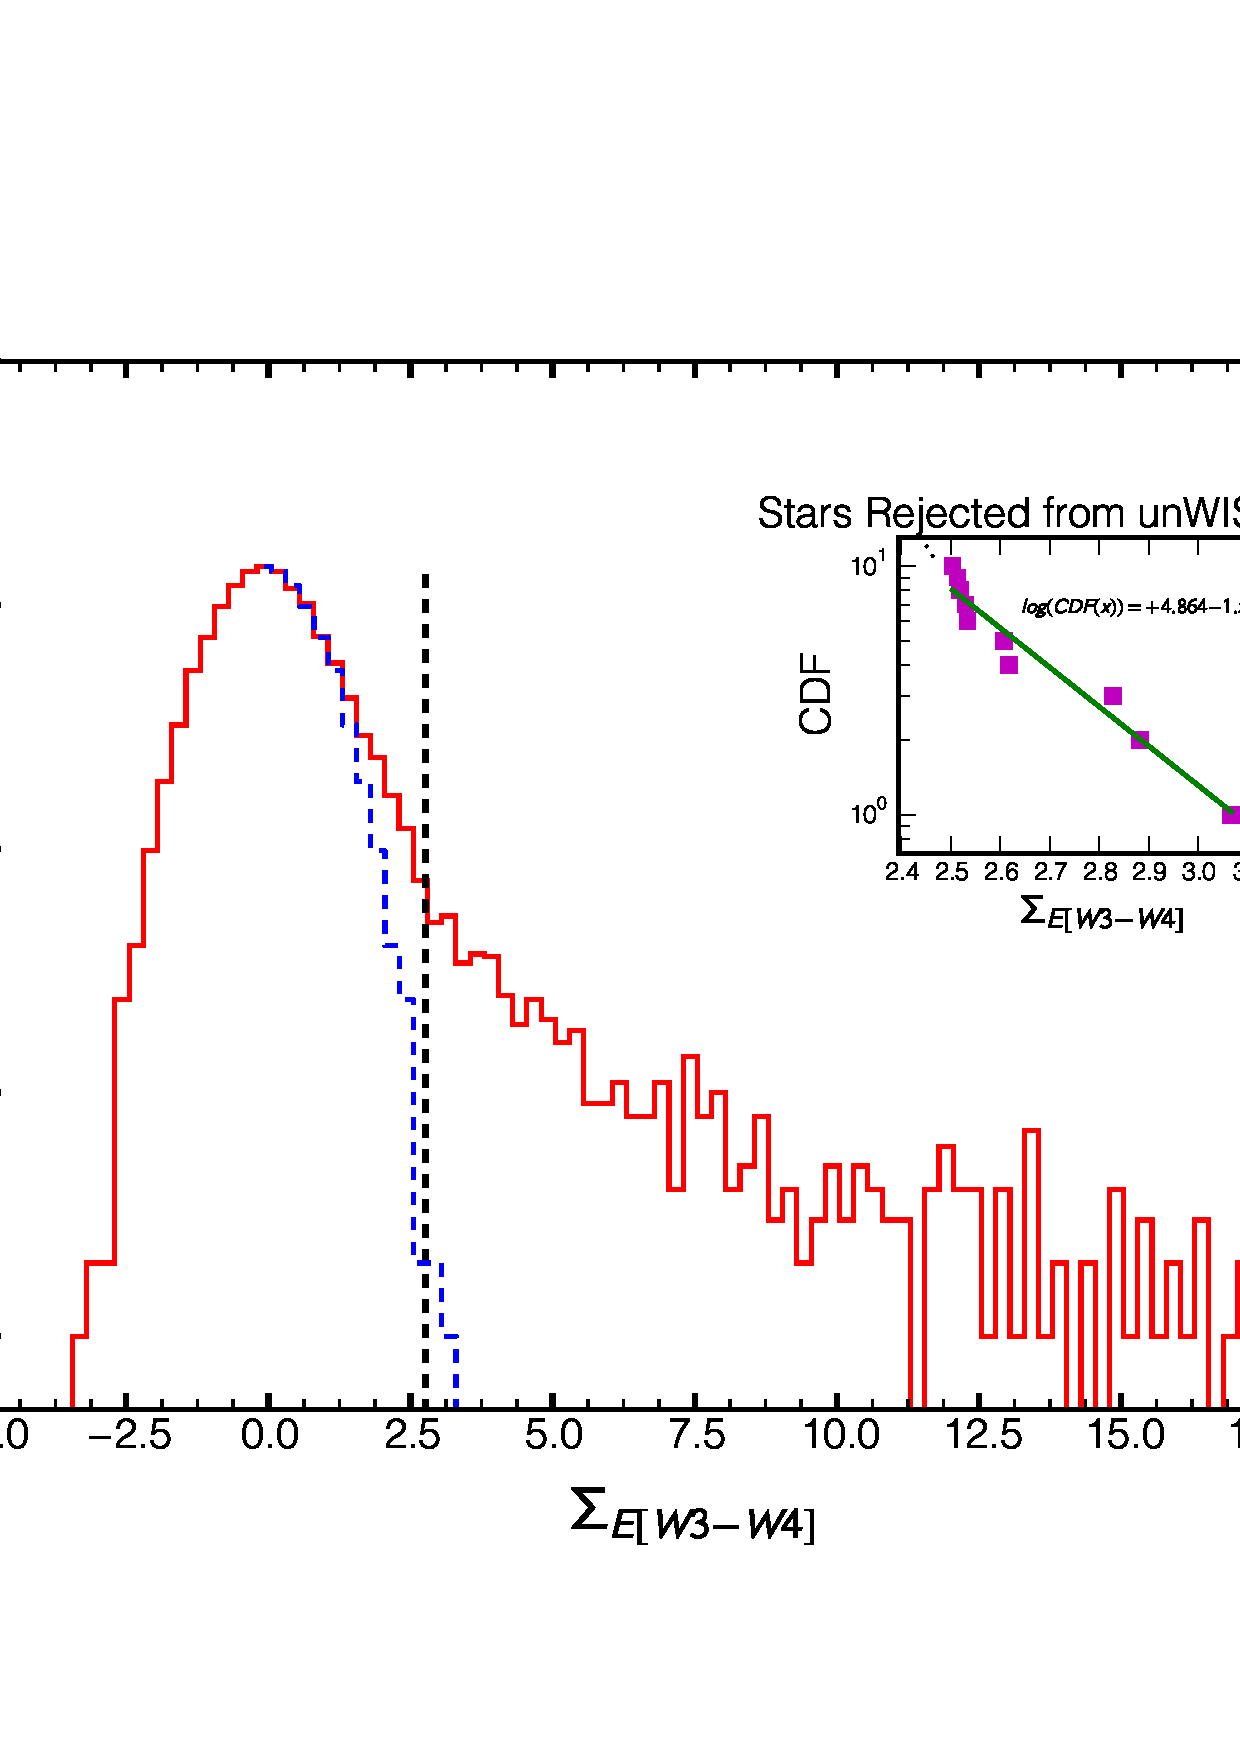
\includegraphics[width=\textwidth]{Ch5/W3-W4_colordist_removedunwisestars_galplane}
    \caption[Distribution of $\Sigma_{E[W3-W4]}$ in 120~pc]{Distribution of $\Sigma_{E[W3-W4]}$ for all our stars in the parent sample (solid red histogram). The blue dashed histogram is the uncertainty distribution, created by reflecting all the values of $\Sigma_{E[W3-W4]}<0$ about the mode of the red distribution. Excesses are selected to the right of our FDR threshold of 0.5\% ($\Sigma_{E[W3-W4]_{99.5}}$), denoted by the vertical dashed green line. This threshold was set at a 99.5\% confidence level. The inset shows a semi-log fit of a line to the last ten points in the reverse cumulative distribution function of the uncertainties. The fit smoothes over the stochasticity in this sparely populated region of the uncertainty distribution to attain a more accurate estimate of the FDR threshold.}
    \label{fig:sige_w3-w4}
    \end{figure}
    %=============================================================

    Our selection process identified 640 stars with significant $W4$ excesses. Out of the 640, we expect 3.2 (=640$\times$0.5\%) of our excesses to be spurious false-positives. In addition, we still need to remove excesses which may be contaminated from interstellar cirrus clouds. Our astrometric offset rejection in \S~\ref{sec:unwise_reject} does not guarantee rejection of all such contaminated stars, as large patches of extended interstellar cirrus may appear as uniform background emission to our centroiding algorithm. Thus, we visually inspected the four band \WS\ Atlas images and removed 119 sources that appear to be contaminated from interstellar cirrus. Since we are using a subset of the parent sample from \citet{Patel2014}, contaminated excesses we rejected in that study appear in this one as well. Therefore, we list the rejected sources in Table~\textbf{XXX}, excluding those which we listed in Chapters~\ref{chap:iddisks} and \ref{chap:confirm}. 
    
    In total, we identified 522 significant $W3-W4$ excesses out to 120~pc. Out of these, 210 were identified by our previous two studies in Chapter~\ref{chap:iddisks} and \ref{chap:confirm}. This leaves 312 stars for which we have not previously reported an excess from our past studies.
    
    \section{Results}
    
    From the 522 debris disks we identified in this study, 16 reside within the galactic plane $|b|<5^{\circ}$. Out of the 312 $W4$ excesses that we had not identified in our previous studies, 225 stars are new 22\micron\ excesses, previously unreported in the literature. Of these, 222 stars do not have previous detection of an excess at any wavelength in the literature. In addition, eight of our new excesses reside within 75~pc. Hence, we are also detecting new excesses within a volume which we had previously searched. 
    
    We also determined the stellar and dust properties of the 522 excess stars, which are listed in Table~\textbf{XXX} and \textbf{XXX}, respectively. We performed the same analysis as in \S~\ref{sec:results} to derive these parameters by performing photospheric model fits. We used NextGen grid models from \citet{Hauschildt1999} to fit the optical and near-IR photometry from \hip\ and \mass. We scaled the derived photospheric model to the mean of the $W1$, and $W2$ photometry. We used the $W4$ excess flux and $W3$ or 3$\sigma$ upper limit to the $W3$ excess flux to determine the best fit blackbody temperature for the dust emission. We have also placed upper limits to all of our dust temperature estimates using the 3$\sigma$ upper limit to the $W3$ excess flux. This allows us to constrain the dust properties to some extent, since we do not have longer wavelength information for all of our stars. Without this information it is difficult to ascertain whether the dust is emitting from warm grains, or whether the excess we measure is the Wien emission of much colder dust. 
    
   % Reuslts:
  %  - # of excesses
  %  - # of new 10--30\micron\ excesses
  %  - # of excesses within gal plane: 16/592 = 2.7\% pm 0.7
  % -- % of stars from parent sample in gal plane: 592/14302 = 4.1% pm 0.2
    %Stars outside galactic plane before unwise: 14433, cut = 2.904
    %stars incluidng galactic plane before unwise: 15199, cut =3.701
    %stars otuside gal plane after unwise: 13710, cut = 2.776
    %stars inside gal plan after unwise: 14302, cut = 2.894
    %-mention how much larger the threshold was if we didn't remove those contaminated stars
    
    %\subsection{Warning of Different Releases}
    %\textbf{Not sure if this should be moved to the discussion section}

\section{Discussion}

    \subsection{Survey Sensitivity}
    
    A goal of this study was to identify faint warm debris disks with \WS, though our detections need to be placed in context to literature excesses. We cannot characterize the full extent of the disk brightness $f_d$ (Equation~\ref{eq:fd}) since we only have excess flux information at $W3$ and $W4$. However, we compare the relative flux at $W4$ ($R_{22}$; Equation~\ref{eq:rel_excess}) of the candidate debris disk hosts from our survey to the relative flux of disks detected at similar wavelengths. Although it would make sense to compare the relative flux of our disks at 22\micron\ to those detected by \iras\ at 25\micron, the latter sample is rather small given that the majority of \iras\ disks were detected in the far-IR. 
    
    %=============================================================
    %  WISE Excess Sensitivity
    %=============================================================
    \begin{figure}
    \centering
    \includegraphics[width=0.85\textwidth]{Ch5/relflux_wise_mips_irs_120pc}
    \caption[Our Survey Flux Sensitivity]{The relative fluxes plotted as a function of their \mass\ $K_s$ magnitudes. The relative fluxes are plotted for our \WS\ excesses from Chapters~\ref{chap:iddisks}, \ref{chap:confirm}, and this study, in addition to stars with 24\micron\ excesses from \citet{Chen2014}, and 32\micron\ \spitzer/IRS excesses from \citet{Lawler2009}. The entire figure extends beyond what is shown. The current limits are set to illustrate the sensitivity limits of each survey.}
    \label{fig:wise_relflux}
    \end{figure}
    %=============================================================
    
    
    Instead, we compare the relative flux at $W4$ for our excesses, to those excesses detected from the \spitzer at 24\micron\ using MIPS. \citet{Chen2014} conducted a study to characterize the excess SEDs of 571 stars with archival \textit{Spitzer}/IRS observations, supplemented with data from observations using \spitzer/MIPS at 24\micron. In addition, \citet{Lawler2009} conducted an unbiased survey to detect Zodiacal light emission from 152 solar type stars in both the \spitzer/IRS short (8.5--12\micron) and long (30--34\micron) bands. We test our sensitivity limits in context to these two surveys: using the relative 24\micron\ flux from \citet{Chen2014} and the relative 32\micron\ flux from \citet{Lawler2009}.
    
    
    
    Figure~\ref{fig:wise_relflux} shows the relative fluxes of the excesses detected from our surveys at 22\micron, excesses with \spitzer/MIPS24 measurements from \citet{Chen2014}, and excesses from \citet{Lawler2009} at 32\micron --- all of them as a function of \mass\ $K_s$ magnitude. What is easily evident is that the \spitzer\ surveys are sensitive to fainter mid-IR excesses compared to \WS. This does not come as a surprise, because \spitzer\ is a pointed telescope. The \spitzer/IRS survey detected dust at 2\% fainter levels compared to the \spitzer/MIPS survey (4\% and 6\% above the photosphere, respectively), mainly because the short wavelength end of the IRS spectra can be used to calibrate the photospheric flux, and use the contemporaneously obtained longer wavelength flux to measure the photospheric flux. 
    
    Our \WS\ excesses, on the other hand, our survey seems to find excesses down to about 9\% of the photospheric emission. This is also of course only for the brightest stars. At fainter stellar magnitudes, the detection sensitivity increases. This is mainly due to the fact that \WS\ is a flux limited survey, and for fainter stars, the photometric uncertainties increase, thereby decreasing the IR excess signal. Thus, this plot tells us that though we are relatively close, we do not do as well as past pointed surveys. 

    %=============================================================
    % My WISE vs. Their WISE
    %=============================================================
    \begin{figure}
    \centering
    \includegraphics[width=.9\textwidth]{Ch5/wise_vs_wu_120pc}
    \caption[My \WS\ Disks vs. Other \WS\ Disks]{Plot of the $B_T-V_T$ colors as a function of the $W3-W4$ color excess ($E[W3-W4]$), for all previously unreported \WS\ $W4$ excesses from our survey, the \WS\ survey by \citet{Vican2014}, and the \WS\ survey by \citet{Wu2013}. The top and right panels show the marginalized distributions of both parameters for all three sets of stars.}
    \label{fig:wise_v_wise}
    \end{figure}
    %=============================================================
    
    However, another picture arises, when comparing our survey to those conducted by others using data from \WS. In Figure~\ref{fig:wise_v_wise}, I plot the $B_T-V_T$ color for the 312 disk candidates we identified from this survey alone, as a function of their $W3-W4$ color excess. In addition, I plot the same parameters for stars that passed our selection criteria, and that were detected by \citet{Vican2014} and \citet{Wu2013}. The division in $B_T-V_T$ between these two surveys is inherent to each, as \citet{Vican2014} searched for excesses around late F to K stars, while \citet{Wu2013} was sensitive to excesses around bright stars A -- F stars. 
    
    What is evident is that the excesses we detect are larger in number, and are detected at fainter levels compared to the other surveys. We cannot rely on the survey results from \citet{Vican2014}, as a number of their stars show negative color excesses or small excesses such that their $\Sigma_{E[W3-W4]}$ are less than our $\Sigma_{E[W3-W4]_{99.5}}$ threshold. These account for $\sim$64\% of the total number of stars in their sample. These excesses were detected by subtracting the photospheric flux after fitting near-IR and optical data to grid models. As we have discussed before, this introduces biases in measuring the excess, and introduces false-positives into the survey. In contrast, our survey is complementary, though larger in scope, to \citet{Wu2013}, as they are preferentially sensitive to brighter excesses. 

    %=============================================================
    %  120 pc incidence rates
    %=============================================================
    \begin{figure}
    \centering
    \includegraphics[width=0.8\textwidth]{Ch5/incidencerates_120pc}
    \caption[Incidence of Excesses]{Fraction of \WS\ $W4$ excesses detected as a function of spectral type in different distance volumes.}
    \label{fig:incidence_rates}
    \end{figure}
    %=============================================================
 
    %=============================================================
    % WISE vs. Literature
    %=============================================================
    \begin{figure}
    \centering
    \includegraphics[width=\textwidth]{Ch5/wise_lit_120pc}
    \caption[Comparison of All Known Debris Disks To Those Detected by \WS]{$B_T-V_T$ colors as a function of distance for all new $W4$ excesses from our three studies, along with debris disks detected at any wavelength in the literature. Marginalized distributions are also plotted on the top and right for each parameter. The grey shaded areas indicate the regions of the parameter space that our surveys do not explore.}
    \label{fig:wise_v_lit}
    \end{figure}
    %=============================================================
    \subsection{Overall Expansion of Disk Census}

    With our large sample size, we can robustly determine the incidence rate of 22\micron\ excesses for a given spectral type. Figure~\ref{fig:incidence_rates} shows the incidence rate of our excesses, as a function of $B_T-V_T$ (spectral type), plotted alongside 1$\sigma$ error bars. We show three different curves, corresponding to the incidence rates for three different volumes, from which we conclude that there does not seem to be any statistically significant deviation as a function of distance. We report a 15--25\% incidence rate of $W4$ excesses for B and A stars, and a 1--4\% incidence for solar type stars (corresponding to an average of 19.0\% and 1.7\%, respectively).


    
    What is even more interesting is how this incidence translates into a total census of disks based on expanding our search to a larger volume. In Figure~\ref{fig:wise_v_lit}, we plot the $B_T-V_T$ of our new \WS\ disks alongside those found in literature (detected at any wavelength) as a function of their distances. The collapsed distance distribution are independent of each other. At distances $<$75~pc, there are clearly a greater number of disks which have been found by other surveys, though our past studies have contributed significantly to the census in this volume. By expanding to 120~pc, we see that within this full volume, we have increased the census of disks by 40\%. However, if we only take the volume of space between 75 and 120~pc, we see that our surveys have increased the census of debris disks by 130\%. 
   


    \subsection{Excesses at False-Discovery Rates $>$ 99.5\%}
    
    We select excesses above $\Sigma_{E[W3-W4]_{34}}$, such that 99.5\% of our stars are bona-fide IR excesses, and not caused by a statistical fluke. However, below this threshold, there are still a non-zero number of bona-fide excesses, at least until the FDR=100\%. The problem is that one cannot lay claim that any particular star below the 99.5\% FDR is a bona-fide excess, give the high rate of contamination. What we can ascertain is how many bona-fide excesses exist below $\Sigma_{E[W3-W4]_{34}}$, by calculating the false omission rate (FOR). The FOR is defined as the number of stars in the uncertainty distribution below $\Sigma_{E[W3-W4]_{34}}$ over the number of stars in the full $\Sigma_E$ distribution below $\Sigma_{E[W3-W4]_{34}}$, but greater than 0. For this study, the FOR = 89.2\%. In other words, 10.8\% of the stars below our threshold, but with $\Sigma_{E[W3-W4]}>0$ are potential bona-fide excesses. In other words, we are insensitive to potentially 724 bona-fide $W4$ excesses, simply due to the width of the uncertainty distribution. 
    
    
\section{Conclusion}
    
    \begin{itemize}
    \item W3-W4 excesses searched out to 120pc and gal plane at 99.5\% confidence
    \item Summary of detections (total stars) and increase of disks (130\%)
    \item Sensitivity level of our survey
    \end{itemize}
   % - visually rejected stars -- more are removed than need be
   
   
\begin{deluxetable}{llc}
\tablewidth{0pt}
\tablecolumns{2}
\tabletypesize{\footnotesize}
\tablecaption{Rejected \WS\ Excesses}

\tablehead{\colhead{HIP} & \colhead{WISE ID}  & \colhead{Rejection} \\ 
           \colhead{ID}       & \colhead{}         & \colhead{Reason}}
\startdata
HIP58   &   J000041.57+621032.7   &   1   \\
HIP2046   &   J002556.62+035531.2   &   1   \\
HIP2415   &   J003047.12+160215.4   &   5   \\
HIP5333   &   J010811.69+550920.5   &   1   \\
HIP7248   &   J013323.57+713316.0   &   1   \\
HIP9018   &   J015607.61+575801.1   &   1   \\
HIP9278   &   J015914.97+670236.4   &   1   \\
HIP10690   &   J021733.88+580111.4   &   1   \\
HIP13460   &   J025318.68+605110.9   &   1   \\
HIP14592   &   J030825.93+570045.5   &   1   \\
HIP15902   &   J032448.99+283908.6   &   1   \\
HIP16459   &   J033201.49+673508.0   &   5   \\
HIP16612   &   J033347.74+521716.5   &   1   \\
HIP16689   &   J033442.86+065035.5   &   1   \\
HIP17575   &   J034550.58+550349.5   &   1   \\
HIP17675   &   J034710.70+514222.3   &   1   \\
HIP17704   &   J034729.46+241717.7   &   1   \\
HIP17886   &   J034932.67+330529.0   &   1   \\
HIP20861   &   J042813.46+450244.6   &   1   \\
HIP21586   &   J043808.01+511009.9   &   1   \\
HIP22306   &   J044815.73+234545.9   &   1   \\
HIP24403   &   J051405.75+211325.3   &   1   \\
HIP25006   &   J052114.72-072847.9   &   1   \\
HIP25197   &   J052327.87+573239.4   &   1   \\
HIP25419   &   J052614.03+164153.6   &   1   \\
HIP25453   &   J052638.83+065206.9   &   1   \\
HIP26560   &   J053852.54+350441.1   &   1   \\
HIP26588   &   J053905.54-055351.3   &   1   \\
HIP28224   &   J055748.66+020356.4   &   1   \\
HIP41690   &   J082955.70-451104.6   &   1   \\
HIP43701   &   J085400.46+201349.4   &   1   \\
HIP48376   &   J095141.32-543935.9   &   1   \\
HIP48627   &   J095457.89-444839.2   &   1   \\
HIP49131   &   J100139.00-552905.8   &   1   \\
HIP54846   &   J111342.81-632411.3   &   1   \\
HIP54854   &   J111350.78-525121.7   &   1   \\
HIP55069   &   J111628.56-603403.8   &   1   \\
HIP55606   &   J112331.01-091521.3   &   1   \\
HIP55909   &   J112735.13-555414.5   &   1   \\
HIP57022   &   J114127.88+005701.0   &   1   \\
HIP57285   &   J114447.30-581553.3   &   1   \\
HIP57291   &   J114450.39-584214.1   &   1   \\
HIP59502   &   J121210.23-632714.8   &   1   \\
HIP59960   &   J121753.15-555831.9   &   1   \\
HIP60068   &   J121903.99-663934.7   &   1   \\
HIP62026   &   J124249.72-555649.2   &   1   \\
HIP62403   &   J124718.84-661414.7   &   1   \\
HIP62538   &   J124853.12-565111.4   &   1   \\
HIP62576   &   J124917.39+273308.9   &   2   \\
HIP63205   &   J125658.67-600835.0   &   1   \\
HIP65100   &   J132030.06-663202.5   &   1   \\
HIP65783   &   J132907.80-644032.9   &   1   \\
HIP66075   &   J133242.44-554939.4   &   1   \\
HIP66632   &   J133928.24-571750.0   &   1   \\
HIP66963   &   J134328.49-543643.7   &   1   \\
HIP67189   &   J134609.32-683357.2   &   5   \\
HIP69011   &   J140740.78-484214.7   &   5   \\
HIP70035   &   J141951.26-611623.5   &   1   \\
HIP70050   &   J142008.31-280256.6   &   5   \\
HIP71585   &   J143824.86-351635.8   &   5   \\
HIP71645   &   J143915.59-642456.9   &   1   \\
HIP74511   &   J151334.72-625639.0   &   1   \\
HIP75134   &   J152112.66-541730.6   &   1   \\
HIP75778   &   J152849.17-535536.4   &   1   \\
HIP76234   &   J153420.83-392057.4   &   5   \\
HIP76782   &   J154037.80-253533.3   &   1   \\
HIP76801   &   J154051.88-292403.2   &   1   \\
HIP77394   &   J154756.48-255913.0   &   1   \\
HIP78085   &   J155639.02-423347.5   &   1   \\
HIP78532   &   J160158.33-465414.2   &   1   \\
HIP78533   &   J160158.85-373203.9   &   1   \\
HIP79026   &   J160747.76-370036.1   &   1   \\
HIP80025   &   J162008.82-361717.1   &   1   \\
HIP80171   &   J162155.29-245929.7   &   1   \\
HIP80770   &   J162927.55-331913.4   &   1   \\
HIP80799   &   J162954.56-245846.5   &   1   \\
HIP81106   &   J163355.15-425320.9   &   1   \\
HIP81467   &   J163820.66-491334.9   &   1   \\
HIP81673   &   J164104.61+361204.1   &   5   \\
HIP83522   &   J170409.70-303936.1   &   1   \\
HIP83711   &   J170629.53-104823.0   &   5   \\
HIP84055   &   J171103.45-313458.7   &   1   \\
HIP84164   &   J171221.84-463352.9   &   5   \\
HIP84359   &   J171448.66-484229.2   &   1   \\
HIP84445   &   J171551.34-301239.1   &   1   \\
HIP86124   &   J173604.59-171822.4   &   5   \\
HIP88460   &   J180341.50-455145.8   &   1   \\
HIP88924   &   J180906.63-092654.7   &   1   \\
HIP89583   &   J181649.60-112423.3   &   1   \\
HIP92973   &   J185627.75-432104.8   &   5   \\
HIP94371   &   J191227.61+165058.4   &   1   \\
HIP95002   &   J191953.09+113206.2   &   1   \\
HIP95696   &   J192751.84+085811.6   &   1   \\
HIP95717   &   J192806.33+175047.7   &   1   \\
HIP98894   &   J200455.18+260311.2   &   1   \\
HIP100767   &   J202551.22+393753.2   &   1   \\
HIP101449   &   J203338.48+532805.6   &   1   \\
HIP103213   &   J205439.94+461352.2   &   1   \\
HIP103269   &   J205516.80+421756.6   &   1   \\
HIP103614   &   J205934.78+611654.4   &   1   \\
HIP103648   &   J210000.36+425552.7   &   1   \\
HIP103994   &   J210411.92-290855.8   &   1   \\
HIP104900   &   J211456.52+642953.3   &   1   \\
HIP105169   &   J211816.29-752048.6   &   1   \\
HIP108414   &   J215747.44-150724.1   &   5   \\
HIP108689   &   J220103.44+555955.3   &   1   \\
HIP109713   &   J221323.87+530914.9   &   1   \\
HIP110214   &   J221931.54+644718.2   &   1   \\
HIP110327   &   J222045.72+560649.6   &   1   \\
HIP116085   &   J233123.69+590957.0   &   1   \\
\enddata
\tablecomments{Rejection reasons:\\
    1. Contamination by nearby infrared source based on visual inspection.\\
    2. Contamination by spectroscopic secondary component.\\
    3. Confusion due to nearby \WS\ source.}
\label{tab:rejects_120}
\end{deluxetable}